\section{One CON frame, line by line}\label{sec:supp-frame}
This section is the line-by-line reading of Section~\ref{sec:worked}.
Listing~\ref{lst:frame} is a complete CON 3.1 file, the survey frame of
a Pt(100) slab of two layers of four atoms with one adatom, written by
readcon-core with velocities.
Table~\ref{tab:frame} gives the content of each line and the rule that
reads it.
The three geometries are Figure~\ref{fig:structures}.
We read the fields in file order, and at each we give what a reader
returns when it gets that field wrong.

% Written by paper/cpc/scripts/survey_listing.py.
\lstinputlisting[numbers=left,numberstyle=\tiny,caption={A Pt(100) slab of two layers of four atoms with one adatom, as one CON 3.1 frame with velocities written by readcon-core \readconCargoVersion{}. Section~\ref{sec:worked} reads it line by line.},label={lst:frame}]{figures/generated/survey_frame.con}


\begin{figure*}[tbp]
\centering
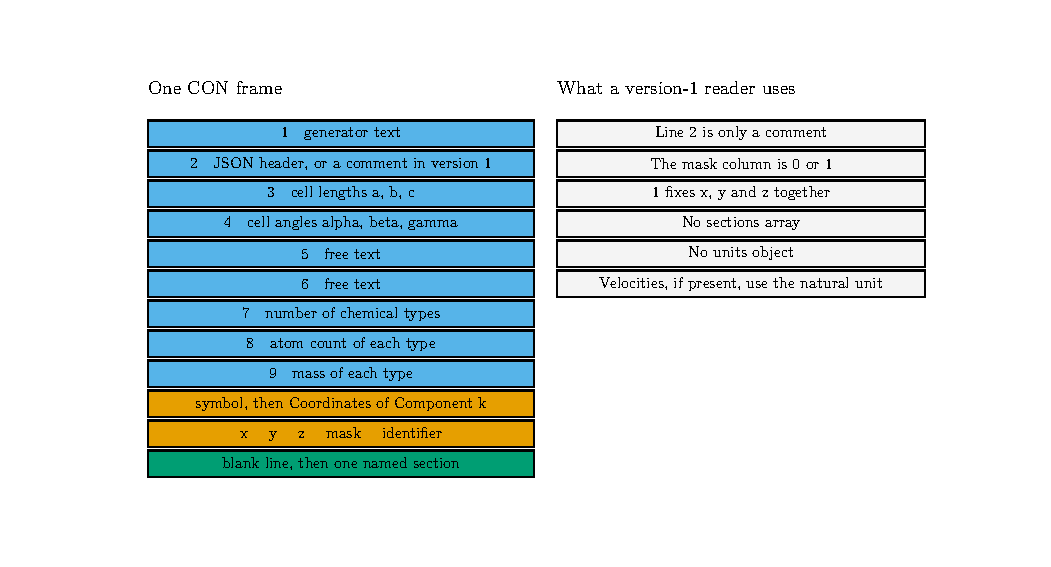
\includegraphics[width=\textwidth]{figures/generated/layout.pdf}
\caption{The lines of one CON frame, and the fields a version-1 reader uses.
The JSON header, the three-bit mask and the identifier are the fields CON 3.1 adds.}
\label{fig:layout}
\end{figure*}


\begin{table}[tbp] \centering \footnotesize \caption{The lines of
Listing~\ref{lst:frame} and the rule that reads each.}
\label{tab:frame}
\begin{tabular}{@{}lp{0.44\linewidth}p{0.36\linewidth}@{}}
\toprule
Line & Content & Rule \\
\midrule
1 & Free text, empty & Kept on rewrite \\
2 & Header: one JSON object with \texttt{con\_spec\_version} 3, \texttt{con\_spec\_minor} 1, \texttt{pbc}, \texttt{sections} and \texttt{units} & Any other header makes the frame version~1 \\
3 & Cell lengths \(a\), \(b\), \(c\) & Eq.~\eqref{eq:cell} \\
4 & Cell angles \(\alpha\), \(\beta\), \(\gamma\) in degrees & Eqs.~\eqref{eq:cell} and~\eqref{eq:gram} \\
5, 6 & Free, empty & Kept on rewrite \\
7 & Atom types, 1 & \\
8 & Atoms of each type, 9 & \\
9 & Mass of each type, \(\wkMass\) amu & \\
\wkLineSymbol & Symbol, \texttt{Pt} & \\
\wkLineCoordinates & \texttt{Coordinates of Component 1} & Labels compare case-insensitively \\
\wkLineFirstRow-{}-\wkLineLastRow & \(x\), \(y\), \(z\), mask, identifier & Mask by Eq.~\eqref{eq:mask}: 7 on the \wkHeldRows{} bottom rows, 0 on the top layer, \wkMaskAdatom{} on the adatom \\
\wkLineBlank & Blank & Opens the declared section \\
\wkLineVelocitySymbol & Symbol, \texttt{Pt} & \\
\wkLineVelocities & \texttt{Velocities of Component 1} & \\
\wkLineFirstVelocity-{}-\wkLineLastVelocity & \(v_x\), \(v_y\), \(v_z\), mask, identifier & In the unit \(\tau\) of Eq.~\eqref{eq:tau} \\
\bottomrule
\end{tabular}
\end{table}

The header line is one JSON object
\cite{brayJavascriptObjectNotation2017}, recognised by its first
non-blank character, \texttt{\{}, and a frame whose header is anything
else is grammar version~1, the text that earlier eOn releases write.
The object of Listing~\ref{lst:frame} names the major and the minor of
the grammar, declares the slab periodic in \(x\) and \(y\) and open in
\(z\), lists \texttt{velocities} as the one section after the
coordinates, and states the units of length, energy, mass and time.

The two cell lines carry the lengths
\(a=b\approx\wkLengthA\,\text{\AA}\) and \(c=\wkLengthC\,\text{\AA}\)
and the angles \(\alpha\), \(\beta\) and \(\gamma\) in degrees, from
which the reader rebuilds the cell with \(\mathbf{a}\) along \(x\) and
\(\mathbf{b}\) in the \(xy\) plane
\cite{bekkerUnificationBoxShapes1997},
\begin{equation}
\label{eq:cell}
\begin{aligned}
\mathbf{a}&=a\,\hat{\mathbf{x}},\qquad
\mathbf{b}=b\cos\gamma\,\hat{\mathbf{x}}+b\sin\gamma\,\hat{\mathbf{y}},\\
\mathbf{c}&=c\cos\beta\,\hat{\mathbf{x}}+c\,\kappa\,\hat{\mathbf{y}}+c\sqrt{\rho}\,\hat{\mathbf{z}},\\
\kappa&=\frac{\cos\alpha-\cos\beta\cos\gamma}{\sin\gamma},\qquad \rho=1-\cos^2\beta-\kappa^2.
\end{aligned}
\end{equation}
The volume is \(V=a\,b\sin\gamma\,c\sqrt{\rho}\), and \(V^2\) is the determinant of the Gram matrix,
\begin{equation}
\label{eq:gram}
\begin{aligned}
\rho\,\sin^2\gamma = D &= 1-\cos^2\alpha-\cos^2\beta-\cos^2\gamma+2\cos\alpha\cos\beta\cos\gamma,\\
\det G &= a^2b^2c^2D .
\end{aligned}
\end{equation}
\(D<0\) is not a cell and \(D=0\) is flat.
Section~\ref{sec:supp-cell} records the right-angle value and the two angle-line variants.
ASE's eon reader stops at the velocity section (line 23).

After two free lines come the counts, one atom type, nine atoms of that
type and the mass of the type, and then a block for each type: its
symbol, a label, and one row of \(x\), \(y\), \(z\), the mask and the
identifier per atom.

For a frame of major \(M\), with \(M=1\) when the header is not JSON,
the mask is the integer
\begin{equation}
\label{eq:mask}
m =
\begin{cases}
b_x + 2 b_y + 4 b_z, & M\ge 2,\\
b_x = b_y = b_z, & M = 1,
\end{cases}
\qquad b_\alpha\in\{0,1\},
\end{equation}
with \(b_\alpha=1\) when component \(\alpha\) is fixed.
The bottom rows of Listing~\ref{lst:frame} are fixed in every component,
the top layer is free, and the adatom is held in \(z\) alone.
A reader that applies the version-1 rule of Table~\ref{tab:clauses} to
this frame rejects the mask of the adatom as an illegal flag, and one
that applies the CON 3.1 rule to a version-1 file frees \(y\) and \(z\)
of every atom held there.
Section~\ref{sec:prefactor} measures what a lost hold of the adatom
changes: the band crosses another saddle, with a larger prefactor.

The identifier is the index of the atom in the numbering of the writer,
from \wkIdFirst{} on the first row to \wkIdLast{} on the last, and
between \wkIdLow{} and \wkIdHigh{} in all.
Grouping by type has permuted that numbering, and ascending identifier
restores it.
A reader returns the identifiers in file order and exactly, up to
\(2^{64}-1\), and a row without an identifier takes its zero-based
position in the frame.
Of the cross-library round trips of Section~\ref{sec:cases}, one returns
no identifiers at all.

The blank line~\wkLineBlank{} opens the velocity section that the header
declared, and the section repeats the block shape with one row of
\(v_x\), \(v_y\), \(v_z\), mask and identifier per atom.
The held atoms have zero velocity and the adatom has \(v_z=0\), so
\wkMovingAtoms{} atoms move.
Their unit is the one the header names, eOn's natural unit,
\begin{equation}
\label{eq:tau}
\tau=\left(\frac{m_{\mathrm{u}}\,\text{\AA}^{2}}{\mathrm{eV}}\right)^{1/2}
=\left(\frac{1.6605\times10^{-27}\,\mathrm{kg}\cdot 10^{-20}\,\mathrm{m}^{2}}{1.6022\times10^{-19}\,\mathrm{J}}\right)^{1/2}
=\wkTimeFs\,\mathrm{fs},
\end{equation}
with the CODATA 2018 values of the atomic mass constant
\(m_{\mathrm{u}}\) and the electronvolt
\cite{tiesingaCodataRecommendedValues2021}.
In that unit the frame has a kinetic energy
\(\tfrac{1}{2}\sum_i m_i\lvert\mathbf{v}_i\rvert^2\) of
\(\wkKinetic\,\mathrm{eV}\).
A reader that takes the same numbers as \(\text{\AA}/\mathrm{fs}\)
returns \(\wkKineticMisread\,\mathrm{eV}\), larger by
\((\tau/\mathrm{fs})^2=\velFactorSq\).

The coordinates are printed in the shortest form that reads back as the
same binary64 value
\cite{steeleHowPrintFloatingpoint1990,adamsRyFastFloattostring2018,clingerHowReadFloating1990}.
Six decimals move the resumed barrier (Section~\ref{sec:supp-cell}).
The frame ends after line~\wkLineLastVelocity, and the next line, if
any, opens the next frame.
Listing~\ref*{lst:testrun} of the supplementary material runs the
example program of the release on this file and on the two variants of
the angle line.



\section{Frame grammar}\label{sec:supp-grammar}
This section is the frame production and the clause list of Section~\ref{sec:format}.
Section~\ref*{sec:spec-normative} of the supplementary material is the
normative specification, \clauseTotal{} numbered clauses, and this
section states the rules that Section~\ref{sec:worked} used, with the
clauses behind them in Table~\ref{tab:clauses}.
A CON file is one or more frames with no marker between them, followed
only by lines of white space.
With \(T\) atom types of \(N_k\) atoms each, a frame \(\mathcal{F}\) is
\begin{equation}
\label{eq:frame}
\begin{aligned}
\mathcal{F}&\to \lambda_1\ \ \lambda_2\ \ (a\ b\ c)\ \ (\alpha\ \beta\ \gamma)\ \ \lambda_5\ \ \lambda_6\ \ T\ \ (N_1\cdots N_T)\\
&\qquad (M_1\cdots M_T)\ \ \mathcal{B}_1\cdots\mathcal{B}_T\ \ \mathcal{S}^{*},\\
\mathcal{B}_k&\to s_k\ \ (\text{\texttt{Coordinates of Component}}\ k)\ \ \bigl(x\ y\ z\ m\ [\iota]\bigr)^{N_k},\\
\mathcal{S}&\to \varnothing\ \ \mathcal{V}_1\cdots\mathcal{V}_T,\\
\mathcal{V}_k&\to s_k\ \ (S\ \text{\texttt{of Component}}\ k)\ \ \bigl(v_1\cdots v_w\ m\ \iota\bigr)^{N_k},
\end{aligned}
\end{equation}
where each symbol or parenthesised group is one line, a superscript
repeats a line, \(\lambda_1\), \(\lambda_5\) and \(\lambda_6\) are free
lines, \(\lambda_2\) is the header, \(M_k\) and \(s_k\) are the mass and
symbol of type \(k\), \(\iota\) is the identifier, \(\varnothing\) is a
blank line and \(S\) is the name of a section of width \(w\).
A type count of zero is a frame without atoms.
The release includes this shape as an informative parsing expression
grammar (PEG) \cite{fordParsingExpressionGrammars2004}, and where the
PEG admits a token that a clause rejects, the clause decides.

Table~\ref{tab:clauses-brief} is the clause list this section uses.
The full clause list, the reserved keys, the reserved sections and the version history are Tables~\ref{tab:clauses}, \ref{tab:keys}, \ref{tab:sections} and~\ref{tab:versions} in the supplementary material.

\begin{table}[tbp] \centering \footnotesize
\setlength{\tabcolsep}{4pt}
\caption{Clauses used in this section.
Tables~\ref{tab:clauses}--\ref{tab:versions} give the full lists.}
\label{tab:clauses-brief}
\begin{tabular}{@{}p{0.22\linewidth}p{0.72\linewidth}@{}}
\toprule
Clause & Rule \\
\midrule
CON-frame.1 & White space after the last complete frame is ignored. \\
CON-token.3 & Fields are separated by spaces and tabs only. \\
CON-cell.3, CON-cell.4 & Without \texttt{pbc} the frame is periodic; a present \texttt{pbc} is three booleans. \\
CON-cell.6 & Without \texttt{lattice\_vectors}, lines 3 and 4 are the cell, angles in degrees. \\
CON-mask.2, CON-mask.3 & In version 1 the mask is 0 or 1. \\
CON-mask.4 & From version 2 the mask is an integer from 0 to 7, Eq.~\eqref{eq:mask}. \\
CON-id.1 & The identifier is an integer from 0 through \(2^{64}-1\), not read through binary64. \\
CON-num.1 & A decimal rounds to the nearest binary64 value. \\
CON-units.8--10 & Before version 3.1 the velocities are in the natural unit; from 3.1 \texttt{units.time} sets that unit. \\
CON-validate.4 & With \texttt{validate} true, a non-positive cell length is rejected. \\
\bottomrule
\end{tabular}
\end{table}


The cell rule rests on Eq.~\eqref{eq:gram}.
readcon-core evaluates Eq.~\eqref{eq:cell} in binary64, accepts the
angles when the computed radicand satisfies
\(\hat\rho>-\num{\wkWindow}\), sets \(c_z=0\) when such a \(\hat\rho\)
is negative, and otherwise rejects the frame as a validation error, a
class that the specification leaves open.
The window is fixed, so it accepts as flat a cell whose exact radicand
lies between \(-\num{\wkWindow}\) and zero, and it rejects every set of
angles that misses a real cell by more.

Table~\ref{tab:clauses} gives the masks that each version admits and the
range of the identifier.
The readcon-core writer refuses a frame that repeats an identifier, and
no clause binds the identifiers of one frame to those of another.

Each number is a finite decimal that the reader rounds to the nearest
binary64 value, ties to even
\cite{ieeecomputersocietyIeeeStandardFloatingpoint2019,clingerHowReadFloating1990,lemireNumberParsingGigabytes2021}.
The default writer prints the shortest decimal that rounds back to the
same value
\cite{steeleHowPrintFloatingpoint1990,loitschPrintingFloatingpointNumbers2010,andryscoPrintingFloatingpointNumbers2016,adamsRyFastFloattostring2018},
so writing a frame and reading it back returns every coordinate
unchanged, and a setting prints six fixed decimals instead.
A gzip or zstd envelope wraps the same text
\cite{deutschGzipFileFormat1996,colletZstandardCompressionApplicationzstd2021},
and a reader recognises it by content.
readcon-core decodes zstd when built with that feature and otherwise
refuses the file by name.

Table~\ref{tab:keys} lists the reserved keys of the JSON line.
The major is \texttt{con\_spec\_version}, and the minor is
\texttt{con\_spec\_minor}, zero when absent.
For a frame whose header is a JSON object, let \(\mu\) be its minor,
\(U\) the set of keys of its \texttt{units} object, and \(V\) true when
the frame has a velocity section.
The reader accepts that header only when
\begin{equation}
\label{eq:version}
\begin{aligned}
&M\in\{2,3\}\ \wedge\ \mu\in\mathbb{N}\\
&\wedge\ \bigl(M=3\Rightarrow\{\mathrm{length},\mathrm{energy}\}\subseteq U\bigr)\\
&\wedge\ \bigl(M=3\wedge\mu\ge1\wedge V\Rightarrow \mathrm{time}\in U\bigr).
\end{aligned}
\end{equation}
For \(M=3\) it also rejects a unit whose dimension is not that of its
quantity.
A reader accepts a later minor of a known major, keeps an unknown key on
rewrite with its digits as read, and rejects any other major as an
unsupported version.
H5MD splits its version into the same pair
\cite{buylH5mdStructuredEfficient2014}.


The sections that \texttt{sections} lists follow the coordinate blocks
in that order, each after one blank line (Table~\ref{tab:sections}).
A section the reader does not know is skipped only when the frame's
minor is later than the reader's and \texttt{section\_arity} gives its
width \(w\ge1\).
Each skipped row has \(w+1\) or \(w+2\) tokens, which the reader counts
without parsing, and any other unknown section rejects the frame.
A frame with no \texttt{sections} key, which includes every version-1
frame, admits a legacy velocity block at its end, a blank line followed
by a complete block of the shape of lines \wkLineVelocitySymbol{}
through \wkLineLastVelocity{} of Listing~\ref{lst:frame}.
Any other blank line there is the first line of the next frame.
The text does not define a blank line, and readcon-core takes it to be a
line of Unicode white space only.
After the last frame it ignores one such line followed by spaces, tabs,
form feeds and line ends.
Table~\ref*{tab:rules-framing} of the supplementary material gives the
other cases.


From minor 1, a frame with a velocity section declares
\texttt{units.time}, and the reader converts that unit to femtoseconds
by Eq.~\eqref{eq:tau}.
Frames of earlier versions are read in the natural unit whatever
\texttt{units.time} names (Table~\ref{tab:clauses}).
Producers of that era wrote natural-unit numbers under an fs label, and
eOn~\eOneEonVersion{} still does
\cite{rohitgoswamiTheochemuieonV3602026}.
The reader keeps such a label without applying it, and a rewrite keeps
the frame at its minor with its label, so the next reader again applies
the natural unit.

Table~\ref{tab:versions} is the history of the grammar.
A change to the text either decides a case that the earlier text left
open, for every version, or adds a requirement under a new minor, which
applies from that minor on.
A later minor therefore never makes a reader reject a file that an
earlier minor requires it to accept.
We take changes through issues and pull requests on the repository, and
each change adds the corpus files that test it.



\section{Path reader and the Python round trip}\label{sec:supp-parser}
This section is the path reader and the Python round trip of Section~\ref{sec:implementation}.
\begin{algorithm}[tbp] \footnotesize \caption{Read a CON file from a
path.}
\label{alg:parser} \begin{algorithmic}[1] \Require path; thread count
\(P\), where absent or 0 selects the default \Ensure frames in file
order, or an error that names its line \State Read the first four bytes;
on gzip magic, decompress every member into memory \State On zstd magic,
decompress when built with zstd, else \textbf{error}: unsupported zstd
input \State Otherwise read a file shorter than \(B_{\mathrm{map}}\)
whole, else memory-map it \If{\(P=1\), or no parallel feature} \State
Parse frame after frame with \Call{ParseFrame}{} \Else \State Walk the
frame boundaries in one thread, skipping each frame by its counts \State
Parse the frames with \Call{ParseFrame}{} in a pool of \(P\) threads, or
the global pool \EndIf \Function{ParseFrame}{} \State \textbf{error} on
a byte-order mark at the start of the file; line 2 is JSON when it
starts with \texttt{\{}, else version 1 \State Check the header against
Eq.~\eqref{eq:version}; keep unknown keys \State Read the cell;
\textbf{error} when \(\hat\rho\le-\num{\wkWindow}\) in
Eq.~\eqref{eq:cell} \State Read the type counts, the masses and the
coordinate rows \State Round each decimal to the nearest binary64 value;
\textbf{error} on a value that is not finite; check each mask against
Eq.~\eqref{eq:mask} \If{line 2 has no \texttt{sections} key} \State Read
a legacy velocity block when a blank line and a complete block follow
\Else \For{each name in \texttt{sections}, in order} \State Read a
reserved section, or count the rows of a later minor's section of
declared width, else \textbf{error} \EndFor \EndIf \State \textbf{error}
on a velocity section without \texttt{units.time} when \(M=3\) and
\(\mu\ge 1\) \EndFunction \end{algorithmic} \end{algorithm}

\begin{lstlisting}[language=Python,caption={\textbf{A checkpoint round trip in Python.} The default printer keeps every binary64 value; six decimals are a separate argument.},label={lst:py}]
import readcon
frames = readcon.read_con("band.con")
readcon.write_con("band.con", frames)
\end{lstlisting}


\section{Claisen drawings}\label{sec:supp-claisen-draw}
These are the drawings cited from Section~\ref{sec:claisen}. Figure~\ref{fig:claisen-land} stays in the main text.
\begin{figure}[tbp]
\centering
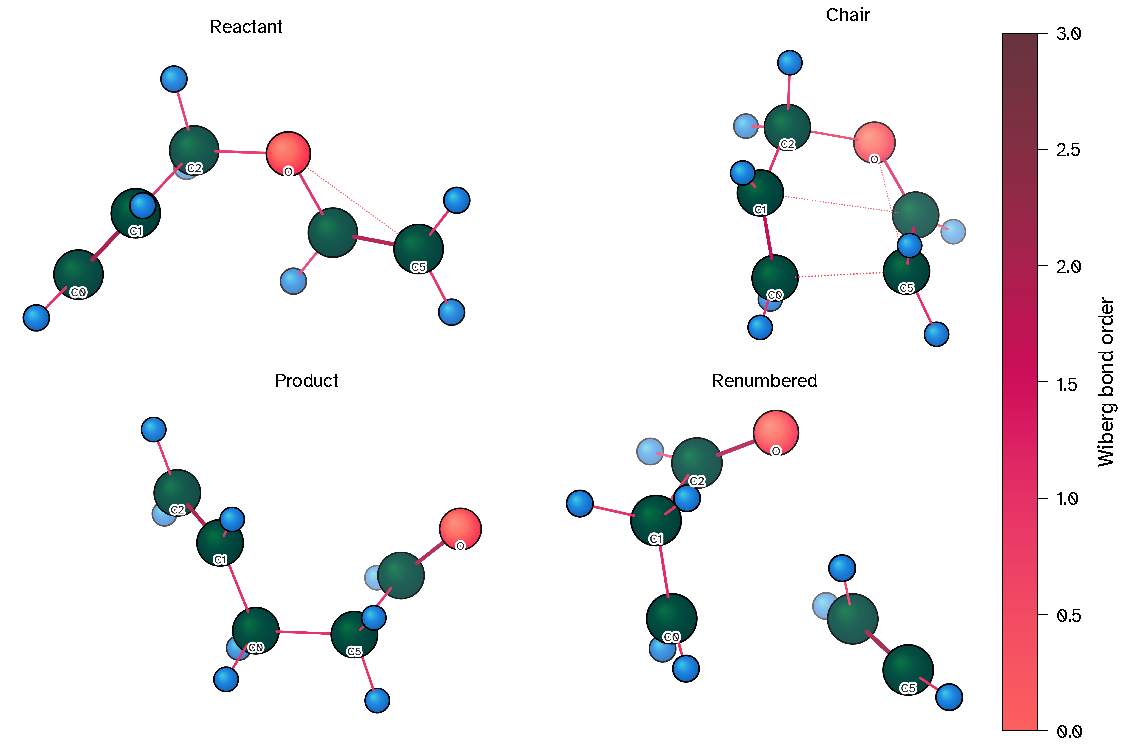
\includegraphics[width=\textwidth]{figures/generated/claisen_wbo.pdf}
\caption{Allyl vinyl ether, the identity-path chair, pent-4-enal, and the highest image of the renumbered band.
Atom colours are the Ruhi palette.
Bond colour and width follow the GFN2-xTB Wiberg bond order, on the scale in the key, and a bond of order below one half is dotted
\cite{wibergApplicationPople1968,bannwarthExtendedTightbindingQuantum2021}.
The drawings are xyzrender
\cite{goodfellowGraphbasedInternalCoordinate2026}.
On the chair the forming C5--C0 contact is the dotted bond, and the breaking C2--O is weakened.
The labelled atoms are C0, C1, C2, C5 and O.
The renumbered image has separated into C0--C1--C2\({=}\)O and C4--C5.}
\label{fig:claisen-struct}
\end{figure}

\begin{figure}[tbp]
\centering
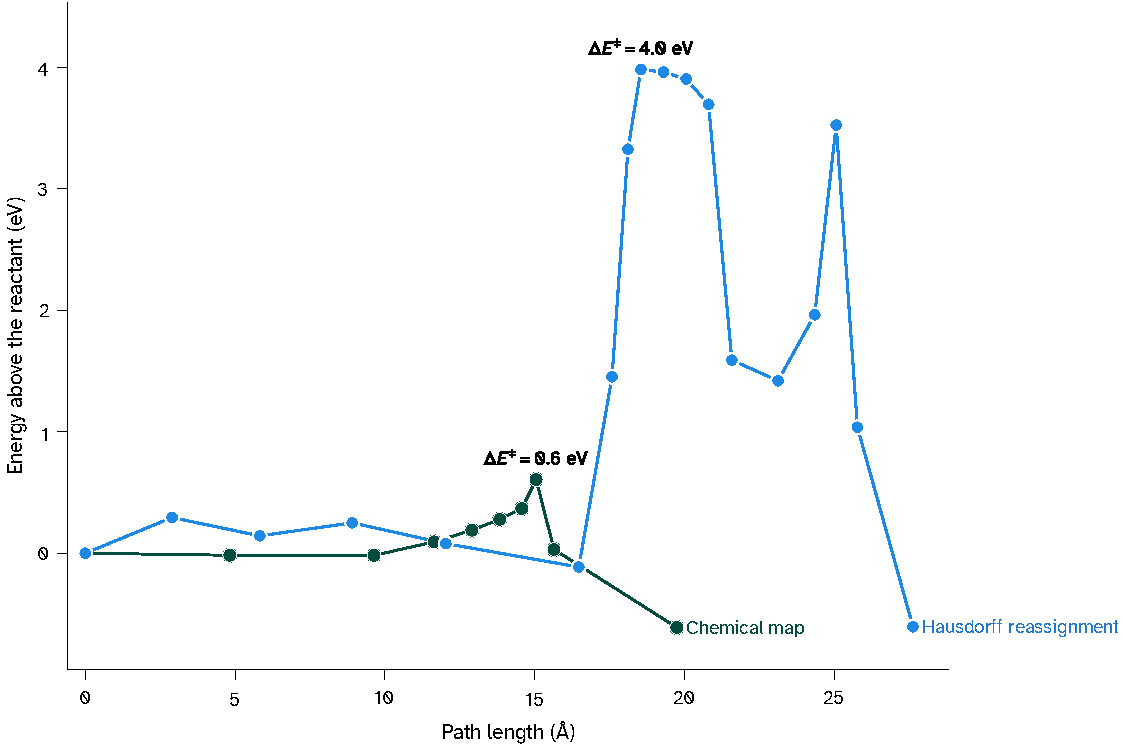
\includegraphics[width=\textwidth]{figures/generated/claisen_neb.pdf}
\caption{Final bands for allyl vinyl ether to pent-4-enal.
Energy of each image above the reactant, joined in path order.
The chemical map follows the atom ids.
The Hausdorff reassignment follows the minimum-Hausdorff permutation of the product.
Each label is the barrier of that band, the highest image above the reactant.
The profiles are drawn with chemparseplot
\cite{goswamiChemparseplot2026}.}
\label{fig:claisen-band}
\end{figure}


\section{Restart tables}\label{sec:supp-restart-tables}
These are the parameter table, the route-by-route band, and the prefactor table of Section~\ref{sec:cases}.
\begin{table}[tbp] \centering \small
\caption{Parameters held fixed for the climbing-image case study.}
\label{tab:params}
\begin{tabular}{@{}llll@{}}
\toprule
Symbol & Meaning & Configuration key & Value \\
\midrule
\(L_{\mathrm{vac}}\) & vacuum on each side of the slab & slab \texttt{vacuum} & \(6.0\,\text{\AA}\) \\
\(z_{\mathrm{ad}}\) & adatom height above the top layer & adsorbate height & \(1.75\,\text{\AA}\) \\
\(f_{\mathrm{end}}\) & endpoint force tolerance & minimise \texttt{fmax} & \(0.002\,\mathrm{eV/\text{\AA}}\) \\
\(f_{\mathrm{band}}\) & band force tolerance & band \texttt{fmax} & \(0.01\,\mathrm{eV/\text{\AA}}\) \\
\(N_{\mathrm{img}}\) & movable images & band images & 5 \\
\(k_{\mathrm{sp}}\) & spring constant & band \texttt{k} & \(0.1\,\mathrm{eV/\text{\AA}^2}\) \\
\(\Delta s\) & steepest-descent step & band step size & \(0.02\,\text{\AA}^2/\mathrm{eV}\) \\
\(K\) & interrupt step & band interrupt & 25 \\
\(N_{\mathrm{cap}}\) & iteration cap & band step limit & 4000 \\
\bottomrule
\end{tabular}
\end{table}

% Written by paper/cpc/scripts/gen_cloud_tables.py.
\begin{table}[tbp]
\centering
\scriptsize
\caption{Resumed climbing-image bands of the EMT Pt(100) adatom hop of Table~\ref{tab:params}, one row per route of the round trip: stopped after 25 steepest-descent steps, written and read back, then resumed to $0.01\,\mathrm{eV}/\text{\AA}$. File is the largest coordinate change on the round trip, and modes are the free Cartesian degrees of freedom of the middle image. Before the write every image carries atom identifiers that are not the row order, each route in its own carrier for them, and kept lists which of the per-component mask, those identifiers, the periodic flags (pbc) and the format version the read returns on every image. Barrier is the highest image energy minus the first, and $\Delta E^\ddagger$ and the displacement are against the uninterrupted band. Force calls count the resumed leg, or the whole band in the uninterrupted row. Wall is the median wall-clock time of that leg alone over 11 interleaved fresh processes, with the interquartile range of those times beside it, so building the band, the first 25 steps and the round trip are outside the clock. POSCAR (ASE), FixScaled z: adatom written T T F. H5MD (h5py), private mask dataset: fixed is not an H5MD element, so only a reader that knows this layout gets the mask back. \textsuperscript{a}29 units in the last place of a 0.009423\,\AA{} coordinate. \textsuperscript{b}21 units in the last place of the 8.771\,eV highest-image energy. \textsuperscript{c}3 units in the last place of a 9.855\,\AA{} coordinate. Section~\ref*{sec:supp-restart} gives the linear-algebra builds on which the printed figures agree.}
\label{tab:restartfmt}
\setlength{\tabcolsep}{2.5pt}
\resizebox{\textwidth}{!}{%
\begin{tabular}{@{}lcccccccccc@{}}
\toprule
Route & File (\AA) & Modes & Kept & Steps & Force calls & Wall (s) & IQR (s) & Barrier (eV) & $\Delta E^\ddagger$ (eV) & Max displacement (\AA) \\
\midrule
uninterrupted & -- & 56 & -- & 60 & 61 & 1.608 & 0.006 & 0.6446 & \num{0} & \num{0} \\
CON 3.1, shortest round trip & \num{0} & 56 & mask, ids, pbc, version & 60 & 36 & 0.955 & 0.007 & 0.6446 & \num{0} & \num{0} \\
CON 3.1, six decimals & \num{4.95e-7} & 56 & mask, ids, pbc, version & 60 & 36 & 0.956 & 0.011 & 0.6446 & \num{1.19e-8} & \num{5.69e-7} \\
extended XYZ (ASE) & \num{4.99e-9} & 56 & mask, ids, pbc & 60 & 36 & 1.008 & 0.006 & 0.6446 & \num{1.09e-9} & \num{4.94e-9} \\
ASE trajectory, ids in tags & \num{0} & 56 & mask, ids, pbc, version & 60 & 36 & 0.951 & 0.006 & 0.6446 & \num{0} & \num{0} \\
POSCAR (ASE), FixScaled z & \num{5e-17}\textsuperscript{a} & 56 & mask & 60 & 36 & 0.965 & 0.007 & 0.6446 & \numrange{-2.0e-14}{3.7e-14}\textsuperscript{b} & \numrange{2.7e-15}{5.3e-15}\textsuperscript{c} \\
H5MD (h5py), private mask dataset & \num{0} & 56 & mask, ids, pbc, version & 60 & 36 & 0.953 & 0.005 & 0.6446 & \num{0} & \num{0} \\
\bottomrule
\end{tabular}}
\end{table}


% Written by paper/cpc/evidence/e5_prefactor.py.
\begin{table}[tbp]
\centering
\scriptsize
\caption{The FIRE climbing-image band of the Table~\ref{tab:restartfmt} slab after each reading of its endpoints. The endpoints are written and read back before they are relaxed, then the band and the Hessians use the constraints that reader returns. Modes and imaginary count the free coordinates of the highest interior image. Before the Hessians are taken, Newton steps on the free coordinates bring the relaxed endpoints to their minima and, where it has one imaginary mode, that image to its saddle. Barrier to four significant figures, prefactor to three.}
\label{tab:prefactor-routes}
\resizebox{\textwidth}{!}{%
\begin{tabular}{@{}llrrrr@{}}
\toprule
Reading & Adatom free & Modes & Imaginary & Barrier (eV) & Vineyard prefactor (Hz) \\
\midrule
height held ($z$ fixed) & x y & 56 & 1 & 0.6446 & \num{9.86e10} \\
height not held & x y z & 57 & 1 & 0.6815 & \num{3.63e12} \\
CON 3.1, shortest round trip & x y & 56 & 1 & 0.6446 & \num{9.86e10} \\
ASE trajectory & x y & 56 & 1 & 0.6446 & \num{9.86e10} \\
POSCAR (ASE), FixScaled $z$ & x y & 56 & 1 & 0.6446 & \num{9.86e10} \\
H5MD (h5py), private mask dataset & x y & 56 & 1 & 0.6446 & \num{9.86e10} \\
\bottomrule
\end{tabular}}
\end{table}



\section{Secondary performance figures}\label{sec:supp-perf-figures}
These are the plain-XYZ reads, the extended XYZ writes and reads, the distributed read, and the database figures of Section~\ref{sec:performance}.
\begin{figure*}[tbp]
\centering
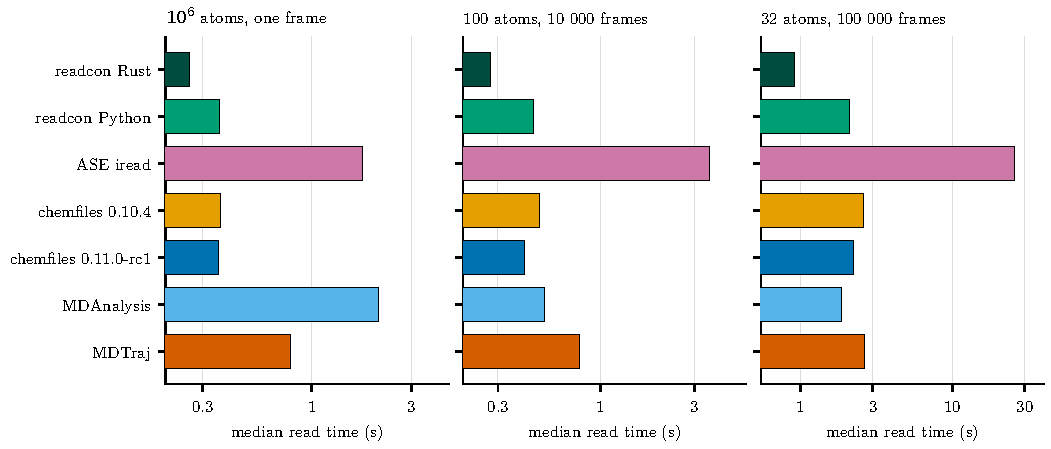
\includegraphics[width=\textwidth]{figures/generated/trajxyz.pdf}
\caption{Median plain-XYZ read against size.
The files are one frame of \(10^{6}\) atoms, \num{10000} frames of 100 atoms, and \num{100000} frames of 32 atoms.
Readers are readcon-core Rust and Python, ASE \texttt{iread}, two chemfiles builds, MDAnalysis and MDTraj.
The axis is logarithmic.}
\label{fig:trajxyz}
\end{figure*}

\begin{table}[tbp]
\centering
\caption{Median extended XYZ write time in seconds.
The files are one frame of \(10^{6}\) atoms and \num{10000} frames of 100 atoms.}
\label{tab:xyzwrite}
\begin{tabular}{@{}lrr@{}}
\toprule
Writer & \(10^{6}\) atoms & \num{10000} frames \\
\midrule
readcon, Rust & 0.487 & 0.431 \\
readcon, Python & 0.442 & 0.411 \\
ASE extxyz & 3.74 & 4.26 \\
ASE cextxyz & 0.948 & 1.47 \\
extxyz 0.4.6 & 0.906 & 1.19 \\
\bottomrule
\end{tabular}
\end{table}

\begin{figure*}[tbp]
\centering
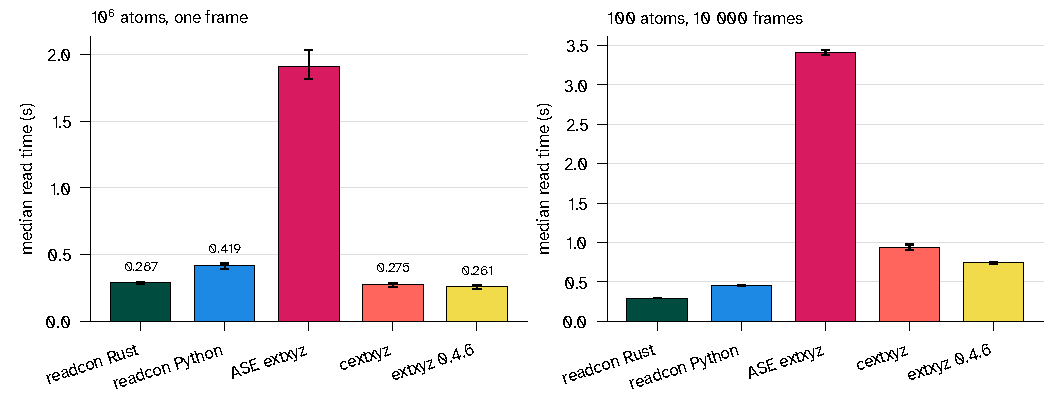
\includegraphics[width=\textwidth]{figures/generated/timings.pdf}
\caption{Median extended XYZ read of the million-atom frame and of the \num{10000}-frame file.
The whisker runs from the first quartile to the third.
On the million-atom frame, extxyz 0.4.6 and cextxyz are faster than readcon.
The resident set and the massif heap of the same reads are Table~\ref{tab:extxyz-h2h}.}
\label{fig:timings}
\end{figure*}

\begin{figure}[tbp]
\centering
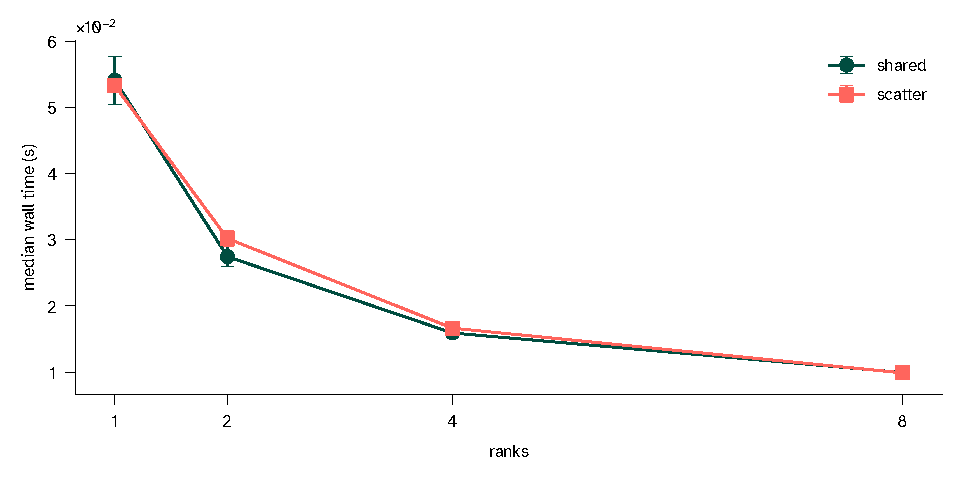
\includegraphics[width=0.85\textwidth]{figures/generated/mpi_host.pdf}
\caption{Distributed read of 4000 frames of 64 copper atoms.
The marker is the type-7 median and the whisker is the type-7 interquartile range.
Shared mode and scatter mode are the two series.}
\label{fig:mpi-host}
\end{figure}

\begin{figure}[tbp]
\centering
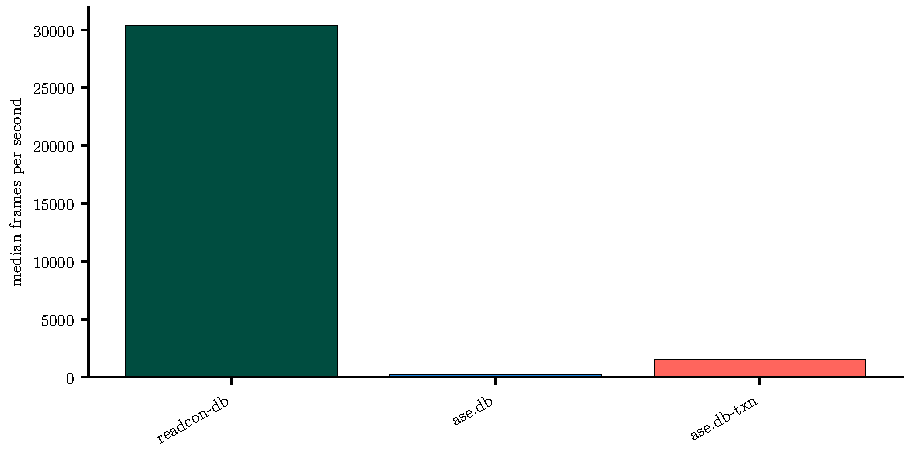
\includegraphics[width=0.72\textwidth]{figures/generated/db_ingest_throughput.pdf}
\caption{Ingest rate on 1000 frames.
The bandwidth and the disk footprint of the same copies are Figures~\ref{fig:db-bandwidth} and~\ref{fig:db-disk}.}
\label{fig:db-throughput}
\end{figure}

\begin{figure}[tbp]
\centering
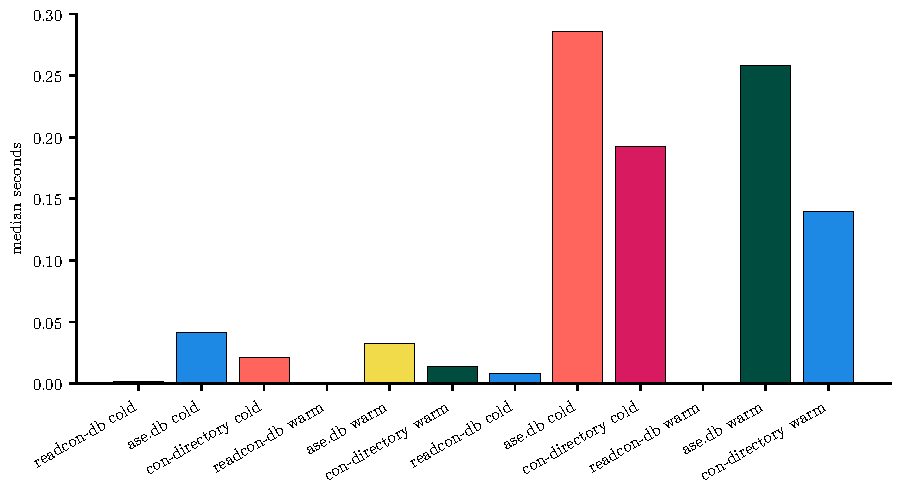
\includegraphics[width=\textwidth]{figures/generated/db_query_latency.pdf}
\caption{Composition-query time on 1000 frames.}
\label{fig:db-query}
\end{figure}


\section{d-SEAMS reader calls}\label{sec:supp-dseams-api}
These are the calls cited from Section~\ref{sec:connectivity}.
The published d-SEAMS analyses read LAMMPS dump text.
seams-core also reads a \texttt{.con} file through readcon-core.
\texttt{sinp::readCon} takes one frame, and \texttt{cloudFromHandle} copies each atom into the point cloud.
\texttt{Point::type} is the atomic number from the file.
\texttt{Point::atomID} is the file's \texttt{atom\_id}.
\texttt{mapAtomIdToIndex} records that id against the cloud index, so a later lookup uses the id and not the row the file happened to write.
A sheared CON cell, lengths and angles, is stored as the same triclinic box a LAMMPS tilt dump carries: the three lengths and the \(xy\), \(xz\) and \(yz\) tilts.

XYZ, as d-SEAMS reads it, has no atom id, so the id is the file order.
Every XYZ atom is stored as type 1, and the comment line is not read as a cell.
A LAMMPS dump carries an id column and a box only when the dump was written with them.
A \texttt{.con} frame carries the id, the element and the triclinic cell on every frame.
A per-atom result then joins the next frame, and a frame in a corpus, by that id.

d-SEAMS uses the LAMMPS dump id for quasi-one-dimensional nanotube water; the same id-to-index map takes the CON \texttt{atom\_id}.
\texttt{ring::rmAxialTranslations} finds the same atom in a later frame through the id-to-index map and shifts the tube along its axis.
The per-atom record is one line of frame, atom id, \(c_{ij}\) and ice type.

readcon-db ingests a \texttt{.con} trajectory into an LMDB corpus.
seams-core selects that corpus by element or by formula, across the shard roots of a campaign, and decodes the \(N\)th hit with the same reader.


\section{Pairing in the dimer, the RMSD and the prefactor}\label{sec:supp-pairing}
This section is the pairing cited from Section~\ref{sec:identity}.
The dimer axis has the same pairing.
With the two images \(R_0\) and \(R_1\),
\begin{equation}
\label{eq:dimer}
\hat N=(R_1-R_0)/|R_1-R_0|,
\end{equation}
and the rotational force is built from the parts of \(-\nabla V(R_1)\) and \(-\nabla V(R_0)\) perpendicular to \(\hat N\)
\cite{henkelmanDimerMethodFinding1999}.
Both \(\hat N\) and that force pair slot \(i\) of \(R_1\) with slot \(i\) of \(R_0\).
The Cartesian RMSD between reactant and product has the same dependence,
\begin{equation}
\label{eq:rmsd}
\mathrm{RMSD}^{2}(R^{\mathrm{R}},R^{\mathrm{P}})=\frac{1}{N}\sum_{a=1}^{N}\big|r_a^{\mathrm{R}}-r_a^{\mathrm{P}}\big|^{2}.
\end{equation}
The sum is a distance between matched atoms.
The permutation-invariant distance minimises Eq.~\eqref{eq:rmsd} over rotations and over the \(M_1!M_2!\cdots\) maps of identical elements
\cite{sadeghiMetricsConfigurationSpace2013,deFindingReactionPathways2019,goswamiTwodimensionalRmsdProjections2026,goswamiChemparseplot2026}.
Two-sided searches need that map before the first image is placed
\cite{deFindingReactionPathways2019,goswamiReproducibleOrchestrationBest2026}.
The image-dependent pair potential builds its target from the distances \(d_{ab}\) of a chosen map and then runs NEB on that objective
\cite{smidstrupImprovedInitialGuess2014}.
A wrong map asks the band to turn the wrong pairs of atoms into neighbours.
Adaptive kinetic Monte Carlo records a process by its saddle.
Two saddles \(R\) and \(R'\) are the same process only when \(|\Pi R-R'|<\epsilon\) for the stored permutation \(\Pi\), and the catalog stores the identity map.
Harmonic transition state theory has the same index: the rate is \(k=\nu\exp(-\Delta E^\ddagger/k_{\mathrm{B}}T)\) with the Vineyard prefactor
\cite{vineyardFrequencyFactorsIsotope1957}
\begin{equation}
\label{eq:vineyard}
\nu=\frac{\prod_{i=1}^{n}\nu_i^{\mathrm{min}}}{\prod_{i=1}^{n-1}\nu_i^{\ddagger}},
\end{equation}
where the products run over the \(n\) free modes of the minimum and the \(n-1\) real modes of the saddle.
Those modes are eigenvectors of the mass-weighted Hessian in the order of \(R\).

\section{Trajectory formats without a per-component mask}\label{sec:supp-formats}
This section is the format comparison cited from Section~\ref{sec:introduction}.
The GROMACS compressed trajectory (XTC) and full-precision trajectory
(TRR) formats \cite{abrahamGromacsHighPerformance2015}, the binary
trajectory (DCD) format of CHARMM
\cite{brooksCharmmBiomolecularSimulation2009} and the trajectory next
generation (TNG) format
\cite{spangbergTrajectoryNgPortable2011,lundborgEfficientExtensibleFormat2014}
store molecular dynamics output with neither a mask nor a velocity unit.
GROMACS deprecates TNG and states that H5MD will replace it, and the
release of 2026-01-19 writes an experimental H5MD trajectory from
\texttt{mdrun} \cite{gromacsManual2026}.
The file handle in that release writes positions, velocities, forces,
the box, the step and the time, and it reads the group
\texttt{/particles/system}.
The H5MD specification it follows still defines no element for a
per-component constraint.

\section{Commands of the companion programs}\label{sec:supp-commands}
This section is the command list of Section~\ref{sec:ecosystem}.
\begin{table}[tbp]
\centering
\caption{Commands of readcon-db and calls of readcon-ops.
readcon-ops has no command line.
The versions and the repositories are in the program summary.}
\label{tab:commands}
\footnotesize
\resizebox{\textwidth}{!}{%
\begin{tabular}{@{}lll@{}}
\toprule
Program & Call & Purpose \\
\midrule
readcon-db & \texttt{ingest} & store a CON trajectory \\
readcon-db & \texttt{select} & return frames by element, formula or topology \\
readcon-db & \texttt{dedup-export} & export unique frames \\
readcon-db & \texttt{annotate-topology} & store the d-SEAMS fingerprint \\
readcon-db & \texttt{find-by-topology} & select by that fingerprint \\
readcon-db & \texttt{shard} & split the corpus \\
readcon-db & \texttt{compact} & reclaim space \\
readcon-db & \texttt{h5md-velocities} & write velocities as H5MD \\
readcon-ops & \texttt{identical} & match atoms of one element under the minimum image \\
readcon-ops & \texttt{internal\_motion} & remove a rigid motion \\
readcon-ops & \texttt{rotational\_match} & align by iterative rotations and assignments \\
\bottomrule
\end{tabular}}
\end{table}

\section{Climbing-image restart protocol}\label{sec:supp-protocol}
This section is the protocol of Section~\ref{sec:cases}.
The restart study
uses a larger slab, Pt(100) under the effective-medium theory (EMT)
potential of ASE \cite{jacobsenSemiempiricalEffectiveMedium1996}, three
layers of \(3\times3\) atoms with the bottom layer held in every
component and one adatom held in \(z\) at the height of
Table~\ref{tab:params} (Figure~\ref{fig:structures}, right).
The adatom hops between neighbouring fourfold hollows along \(x\).
With the slab fixed, the EMT force on the adatom at that height exceeds
the band tolerance.
That height is no stationary point of the free adsorbate, so a file that
drops the hold resumes another relaxation.
A climbing-image band of five movable images with the improved tangent
\cite{henkelmanClimbingImageNudged2000,henkelmanImprovedTangentEstimate2000}
converges under fixed-step steepest descent on the projected force,
which keeps no step history, so a difference after the restart comes
from the file.
The spring and the tangent are the defaults of ASE, the band tolerance
is the default force tolerance of the ASE optimiser divided by the five
movable images, and each endpoint is minimised to that tolerance divided
by five again \cite{larsenAtomicSimulationEnvironmenta2017}.
A force equal to the band tolerance moves an atom by
\(2\times 10^{-4}\,\text{\AA}\) under that step.
Uninterrupted, the band converges in \(\rfStepsUnint\) steps and
\(\rfCallsUnint\) force calls, with barrier
\(\rfBarrierUnint\,\mathrm{eV}\) and \(\rfModesUnint\) free modes on the
middle image.
We interrupt it after \(K\) steps, write it, read it back and resume it
to \(f_{\mathrm{band}}\), once per route of Table~\ref{tab:restartfmt}.

\section{Second corpus, independent reader and per-path checks}\label{sec:supp-corpora}
This section is the conformance detail of Section~\ref{sec:conformance}.
That corpus has few files for the header, the sections and the units, so
we wrote a second corpus of \(\cthreeoneFiles\) CON 3.1 files,
\(\cthreeoneAccepted\) legal and \(\cthreeoneRejected\) illegal.
Its manifest names for each file the clauses that decide it and the
outcome, the frame count and periodic flags of a legal file or the error
class and line of an illegal one.
For \(\cthreeoneExplicit\) entries the outcome follows from the text of
a clause, and the others record a reading where the text leaves a case
open (Section~\ref*{sec:supp-corpus31}).
All \(\cthreeoneMatch\) files return the outcome of their entry at one,
two and eight threads and at the default.
Both corpora also go through every read path of the Python module and
the C library, in the default and the parallel build at each of those
thread counts, and all \(\cpathsReads\) reads return the outcome that
the manifests name (Table~\ref*{tab:corpus-paths}).

We also wrote an independent reader in \(\corpusIndepLines\) Python
source lines that import nothing from readcon.
It follows the clauses of the specification, and where a clause requires
a rejection without naming its class, or no clause decides a case, it
follows the reading of the corpus manifest.
Of the \(\corpusFiles\) files of both corpora, the frame list and the
frame iterator of readcon and the independent reader each return the
manifest outcome on all \(\corpusIndepAgree\).
On the \(\corpusBoth\) files that both readers accept, all
\(\corpusFieldIdentical\) carry the same bits in every coordinate,
velocity and cell entry and equal masks, identifiers, units and periodic
flags (Table~\ref*{tab:corpus-crosscheck}).
The two readers also read \(\mutantCases\) mutants of the
\(\mutantFiles\) corpus files.
They agree on \(\mutantSame\) of them.
The count-line rule accounts for all 15 differences.
The release runs 140 differential cases.
Of the \(\clauseTotal\) clauses of the specification, \(\clauseCovered\)
are named by a corpus file, a probe or a test of the library, and the
other \(\clauseUncovered\) state no duty of a reader.

\section{Atom-id calls}\label{sec:supp-api}
This section is the call table of Section~\ref{sec:implementation}.
\begin{table}[tbp]
\centering
\caption{The four atom-id calls of the released API in readcon-core 0.21.0.
In C++ the consistency check is the free function.
The other three C++ calls are members of \texttt{ConFrame}.}
\label{tab:correspondence}
\footnotesize
\resizebox{\textwidth}{!}{%
\begin{tabular}{@{}lll@{}}
\toprule
Python & C & C++ \\
\midrule
\texttt{atom\_id\_permutation} & \texttt{rkr\_frame\_atom\_id\_permutation} & \texttt{ConFrame::atom\_id\_permutation} \\
\texttt{reorder\_like} & \texttt{rkr\_frame\_reorder\_like} & \texttt{ConFrame::reorder\_like} \\
\texttt{check\_atom\_id\_consistency} & \texttt{rkr\_frames\_check\_atom\_ids} & \texttt{check\_atom\_id\_consistency} \\
\texttt{minimum\_image\_displacements} & \texttt{rkr\_frame\_minimum\_image\_displacements} & \texttt{ConFrame::minimum\_image\_displacements} \\
\bottomrule
\end{tabular}}
\end{table}

\section{Hausdorff renumbering of the Claisen product}\label{sec:supp-claisen-protocol}
This section is the renumbered-band protocol of Section~\ref{sec:claisen}.
IRA reassigns the same product by the rotation and the permutation that minimise the Hausdorff distance, with \(k_{\max}\) factor 3
\cite{gundeIRAShapeMatching2021}.
The permutation is \([0,4,3,1,2,5,6,7,11,12,13,9,8,10]\), and it moves 10 of the 14 atoms.
The Hausdorff distance is \(2.109\,\text{\AA}\).
Equation~\eqref{eq:rmsd} after the Kabsch rotation is \(1.443\,\text{\AA}\) on this map and \(1.519\,\text{\AA}\) on the identity map.
The shorter distance pairs the wrong nuclei for the [3,3] shift.
A single point on the relabelled product is \(-81.432\,\mathrm{eV}\), against \(-81.439\,\mathrm{eV}\) on the identity product: the same molecule, rigidly moved, so the endpoints are equivalent and only the labelling differs.

That labelling was first run with the setup of the identity band: eight images between the endpoints, ten images in the band, an S-IDPP start
\cite{smidstrupImprovedInitialGuess2014}, and the published climbing-image settings.
The climbing image oscillated, and the band did not converge.
The same labelling was then given sixteen images between the endpoints, eighteen in the band, a maximum step of \(0.05\,\text{\AA}\) against \(0.1\,\text{\AA}\), and a cap of 2000 iterations against 1000, with the climber held on (Figure~\ref{fig:claisen-band}, Figure~\ref{fig:claisen-land}).
Figure~\ref{fig:claisen-land} is the plane of \(s\) and \(d\), the RMSD-based reaction progress and the orthogonal deviation of the MethodsX projection, drawn with chemparseplot
\cite{goswamiTwodimensionalRmsdProjections2026,goswamiChemparseplot2026}.
The band force reached \(0.189\,\mathrm{eV/\text{\AA}}\) at iteration 362 and no lower.
A further climbing-image-only continuation oscillated between about \(0.19\,\mathrm{eV/\text{\AA}}\) and several \(\mathrm{eV/\text{\AA}}\) and did not reach \(0.05\,\mathrm{eV/\text{\AA}}\).
Neither setup meets the \(0.05\,\mathrm{eV/\text{\AA}}\) criterion.
The highest image of the eighteen-image band lies at 3.988~eV (92.0~kcal/mol).
The atoms have separated into C0--C1--C2\({=}\)O and a detached C4--C5, with O--C4 at \(2.874\,\text{\AA}\) (Figure~\ref{fig:claisen-struct}).
Three internal modes are imaginary, at \(-251\), \(-135\) and \(-123\,\mathrm{cm}^{-1}\).
The image is a higher-order stationary point.
The images of Eq.~\eqref{eq:lerp} on this permutation drag atoms through one another, because a slot in \(R^{\mathrm{P}}\) holds a different nucleus from the slot in \(R^{\mathrm{R}}\).

\section{Water quench}\label{sec:supp-water-protocol}
This section is the trajectory protocol of Section~\ref{sec:connectivity}.
The system is mW water, 4096 molecules
\cite{molineroWaterModeledIntermediate2009}, equilibrated in the NVT ensemble at 350~K and then quenched in the NVT ensemble at 180~K, with a 10~fs step and a 200~fs damping time, in the LAMMPS build of 22~July~2025
\cite{thompsonLammpsFlexibleSimulation2022}.
An 81-frame window, from 659~ps to 739~ps after the quench, brackets the frame at 705~ps in which a 50-molecule CHILL+ ice core is present
\cite{nguyenIdentificationClathrateHydrates2015}.
The neighbour cutoff is \(3.5\,\text{\AA}\), primitive rings are counted up to seven members, and the ice label is the CHILL+ class, the published d-SEAMS settings
\cite{goswamiDseamsDeferredStructural2020}.
The same frames were written as CON and as XYZ.
A LAMMPS dump written without \texttt{dump\_modify sort} lists atoms in per-processor order, and that order changes as atoms migrate between subdomains.
The XYZ order, permuted independently in every frame, stands for that listing and for any writer that reorders atoms.
Both analyses use the same orthorhombic cell: the three lengths of the dump box and right angles, stored on the CON frame and repeated on the XYZ comment line.

\section{The five restart requirements}\label{sec:supp-requirements}
This section states the requirements of Table~\ref{tab:requirements}.
R1 is a mask for each Cartesian axis of each atom.
R2 is an integer stored on the row, so a later frame finds the same atom after the file groups rows by element.
R3 is a time unit written in the file.
R4 is coordinates, cell and periodic flags that read back as the values written.
R5 is a grammar with a major and a minor, a rule for what a later minor may add, and a corpus that decides disputes.
The short history of an optimiser is outside the five.
Limited-memory quasi-Newton updates a Hessian from a few previous steps \cite{nocedalUpdatingQuasinewtonMatrices1980}.
The optimisers used on minimum-energy paths keep an analogous history \cite{sheppardOptimizationMethodsFinding2008}.
FIRE carries velocities of the images between steps \cite{bitzekStructuralRelaxationMade2006}.
A resume can match the coordinates and still take a different next step.

\section{What each format keeps}\label{sec:supp-fields}
This section is the field-by-field comparison of Section~\ref{sec:fields}.
Column 5 is the atom id, and it holds the original index.
A rewrite that groups the rows by element recovers that order from the column.
ASE's eon reader ignores the column
\cite{larsenAtomicSimulationEnvironmenta2017}.
Plain XYZ has no id column.
Extended XYZ carries one only under ASE's column name, which no grammar reserves
\cite{kermodeLibatomsExtxyzV0462026} (Table~\ref{tab:spec-compare}).
A LAMMPS dump and an H5MD file can carry one
\cite{thompsonLammpsFlexibleSimulation2022,buylH5mdStructuredEfficient2014}.
readcon keeps \texttt{atom\_id} through the read and the write, so the identity survives the reordering.
A NEB band, a dimer and an AKMC comparison of images need that identity.

Column 4 is a per-axis mask, an integer from 0 to 7, Eq.~\eqref{eq:mask}.
The mask removes Cartesian components from the free set \(n\) in Eq.~\eqref{eq:vineyard}.
A constrained dimer or a constrained band holds those components fixed.
On the Pt(100) adatom the held height selects one saddle.
Dropping the hold selects another, \(0.68\,\mathrm{eV}\) with a prefactor 37 times larger (Section~\ref{sec:prefactor}).
ASE's eon reader passes the column through \texttt{bool}, and its writer emits only 0 or 1, so a mask on one axis is stored as a hold on all three.
Extended XYZ and H5MD have no element for the mask.
POSCAR stores it as selective dynamics
\cite{vaspwikiPoscar2026}.
The ASE bridge in readcon writes a partial mask back as the same integer.

The mass \(m_a\) is stored on the atom.
The Lagrangian of the nuclei is
\begin{equation}
\label{eq:lagrangian}
L=\sum_{a=1}^{N}\tfrac12 m_a|\dot r_a|^{2}-V(R).
\end{equation}
A ring-polymer instanton discretises a periodic path in imaginary time, and the action weights each bead by the same masses
\cite{richardsonRingpolymerInstanton2018}.
XTC, TRR and DCD keep those masses in a separate topology file
\cite{abrahamGromacsHighPerformance2015,brooksCharmmBiomolecularSimulation2009}.
The cell of the frame is the \(3\times 3\) matrix used for the minimum image inside \(|R_{i+1}-R_i|\).

A velocity \(v_a\) is the momentum in Eq.~\eqref{eq:lagrangian} divided by \(m_a\).
The velocities occupy a declared section, and the reader uses the time unit that section names.
Archived eOn documents its natural unit as the constant \(\velEonFs\,\mathrm{fs}\).
The same digits read as \(\text{\AA}/\mathrm{fs}\) scale the kinetic energy by \(\velFactorSq\), Eq.~\eqref{eq:tau}.
ASE's eon writer writes no velocities.

From version 3.5, eOn reads CON through readcon
\cite{chillEonSoftwareLong2014,rohitgoswamiTheochemuieonV3602026}.
The ase-readcon plugin registers the formats \texttt{readcon-con} and \texttt{readcon-convel}.
The readcon-chemfiles bridge reads XYZ, PDB, GRO and LAMMPS dump text into a \texttt{ConFrame}
\cite{frauxChemfileschemfilesVersion01042023}.
Residue records and per-atom properties that are not CON columns are left out of that frame.

\section{eOn resuming a Morse band}\label{sec:supp-morse}
This section is the Morse restart of Section~\ref{sec:eon-band}.
The public eOn client resumes from its own output files.
The default band optimiser of eOn is the limited-memory form, L-BFGS, of
the Broyden, Fletcher, Goldfarb and Shanno update
\cite{nocedalUpdatingQuasinewtonMatrices1980,sheppardOptimizationMethodsFinding2008},
and its memory vectors are stored in no geometry file.
A restart therefore cannot repeat an L-BFGS path from the geometry alone.
The uninterrupted Morse band, on eOn's Morse potential, takes 946 optimiser steps and 4737 force calls, and the barrier is 1.37~eV (Figure~\ref{fig:restart}).
The round trip reaches the same barrier, with a shift of 0, in 922 optimiser steps and 4617 force calls on the resumed leg.
Six decimals shift the barrier by \(1.00\times 10^{-6}\)~eV and take the same resumed leg.
